\documentclass[11pt, oneside]{article}
\usepackage{amsmath}
\usepackage{amssymb}
\usepackage[usenames,dvipsnames]{xcolor}
\usepackage{tikz}
\usepackage{xcolor}
\usetikzlibrary{snakes}
\usetikzlibrary{decorations}
\usetikzlibrary{trees}
\usetikzlibrary{decorations.pathmorphing}
\usetikzlibrary{decorations.markings}
\usetikzlibrary{external}
\usetikzlibrary{intersections}
\usetikzlibrary{shapes,arrows}
\usetikzlibrary{arrows.meta}
\usetikzlibrary{calc}
\usetikzlibrary{shapes.misc}
\usetikzlibrary{decorations.text}
\usetikzlibrary{backgrounds}
\usetikzlibrary{fadings}
\usepackage{tikz}
\usetikzlibrary{patterns}
\usetikzlibrary{positioning}
\usetikzlibrary{tikzmark,calc,arrows,shapes,decorations.pathreplacing}
\tikzset{
        cross/.style={cross out, draw=black, minimum size=2*(#1-\pgflinewidth), inner sep=0pt, outer sep=0pt},
	branchCut/.style={postaction={decorate},
		snake=zigzag,
		decoration = {snake=zigzag,segment length = 2mm, amplitude = 2mm}	
    }}

\begin{document}

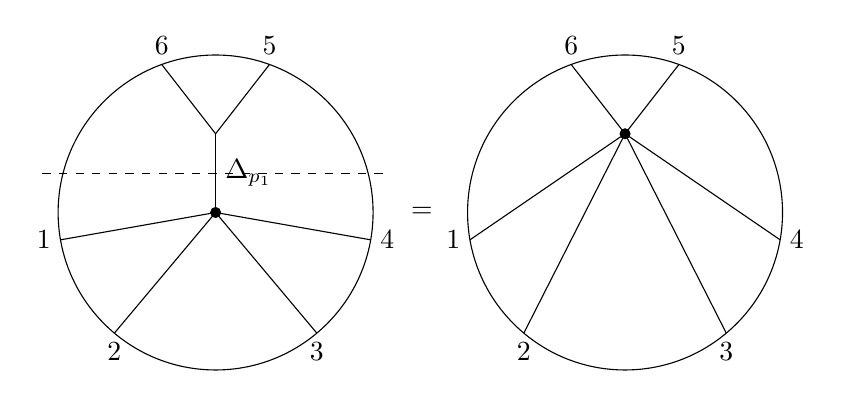
\begin{tikzpicture}
        % Circle boundary
        \draw (0,0) circle (2 cm);
        
        % Points
        \coordinate (1) at (-1.96962,-0.347296);
        \coordinate (2) at (-1.28558,-1.53209);
        \coordinate (A) at (-2.2,0.5);
        \coordinate (B) at (2.2,0.5);
        \coordinate (C) at (0,0);
        \coordinate (D) at (0,1);
         \coordinate (3) at (1.28558,-1.53209);
        \coordinate (4) at (1.96962,-0.347296);
          \coordinate (5) at (0.68404,1.87939);
        \coordinate (6) at (-0.68404,1.87939);
              
        % Lines connecting points
        \draw (1) -- (C);
        \draw (2) -- (C);
       \draw (3) -- (C);
        \draw (4) -- (C);
        \draw (5) -- (D);
        \draw (6) -- (D);
        \draw (D) -- (C) node[midway, right] {\(\Delta_{p_1}\)};
        \draw[dashed] (A) -- (B);
                  
        % Points
        \fill (1)  node[left] {$1$};
        \fill (2) node[below] {$2$};
        \fill (3) node[below] {$3$};
         \fill (4) node[right] {$4$};
          \fill (5) node[above] {$5$};
         \fill (6) node[above] {$6$};
         \fill (C) circle (2pt);
         \node[anchor=west, right=2.3 cm of C] (formula) {\(\,=\)};  
          % Circle boundary
        \draw (5.2,0) circle (2 cm);
        
        % Points
        \coordinate (1p) at (3.23038,-0.347296);
        \coordinate (2p) at (3.91442,-1.53209);
        \coordinate (Dp) at (5.2,1);
         \coordinate (3p) at (6.48558,-1.53209);
        \coordinate (4p) at (7.16962,-0.347296);
          \coordinate (5p) at (5.88404,1.87939);
        \coordinate (6p) at (4.51596,1.87939);
              
        % Lines connecting points
        \draw (1p) -- (Dp);
        \draw (2p) -- (Dp);
       \draw (3p) -- (Dp);
        \draw (4p) -- (Dp);
        \draw (5p) -- (Dp);
        \draw (6p) -- (Dp);                  
        % Points
        \fill (1p)  node[left] {$1$};
        \fill (2p) node[below] {$2$};
        \fill (3p) node[below] {$3$};
         \fill (4p) node[right] {$4$};
          \fill (5p) node[above] {$5$};
         \fill (6p) node[above] {$6$};
         \fill (Dp) circle (2pt);
       \end{tikzpicture}

\end{document}